\documentclass[a4paper]{article}

\usepackage{afterpage}
\usepackage{bold-extra}
\usepackage{color}
\usepackage{float}
\usepackage{graphicx}
\usepackage{listings}
\usepackage{subfigure}
\usepackage{url}

%%%%%%%%%%%%%%%
%%% Colours %%%
%%%%%%%%%%%%%%%

\definecolor{darkgreen}{rgb}{0, 0.6, 0}
\definecolor{lightgrey}{gray}{0.9}

%%%%%%%%%%%
% Figures %
%%%%%%%%%%%

% Define shorter ways to include individual images
\newcommand{\stufig}[4]						% images with default placement
{
	\begin{figure}
	\begin{center}
		\includegraphics[#1]{#2}
		\caption{#3}
		\label{#4}
	\end{center}
	\end{figure}
}

\newcommand{\stufigex}[5]					% images with specified placement
{
	\begin{figure}[#5]
	\begin{center}
		\includegraphics[#1]{#2}
		\caption{#3}
		\label{#4}
	\end{center}
	\end{figure}
}

\newcommand{\stufigexx}[5]				% full-width images with specified placement
{
	\begin{figure*}[#5]
	\begin{center}
		\includegraphics[#1]{#2}
		\caption{#3}
		\label{#4}
	\end{center}
	\end{figure*}
}

% Define the stusubfig environment
\newenvironment{stusubfig}[1]
{
	\begin{figure*}[#1]
	\begin{center}
}
{
	\end{center}
	\end{figure*}
}

%%%%%%%%%%%%%%%%%
% Code Listings %
%%%%%%%%%%%%%%%%%

% Create a new type of float (called a stulisting) for listings
\floatstyle{ruled}
\newfloat{stulisting}{thp}{lop}
\floatname{stulisting}{Listing}

% Setup before using the listings package
\renewcommand{\lstlistingname}{\textbf{Listing}}
\def\thelstlisting{\textbf{\arabic{lstlisting}}}

\lstdefinelanguage{Pseudocode}{
morekeywords={and,assert,break,case,continue,default,down,each,else,for,function,if,not,null,or,rangeswitch,ref,return,switch,then,this,throw,to,up,var,while},
sensitive=true,
morecomment=[l]{//},
morecomment=[s]{/*}{*/}
}

\lstdefinestyle{Default}{
abovecaptionskip=0.5cm,
basicstyle=\scriptsize\ttfamily,
belowcaptionskip=0.5cm,
belowskip=0.5cm,
columns=fixed,
%commentstyle=\color{darkgreen},
commentstyle=\textit, % changed from the thesis (green text looks unprofessional in a journal paper)
language=Pseudocode,
%numbers=left,
numbers=none, % changed from the thesis (line numbers are less relevant here)
numbersep=5pt,
numberstyle=\tiny,
mathescape=true,
showstringspaces=false,
stepnumber=1,
tabsize=4
}

\lstdefinestyle{Snippet}{
abovecaptionskip=0.5cm,
aboveskip=0.5cm,
basicstyle=\small\ttfamily,
belowcaptionskip=0.5cm,
belowskip=0.5cm,
columns=fixed,
commentstyle=\color{darkgreen},
frame=lines,
keywordstyle=\small\bfseries,
language=Pseudocode,
numbers=none,
mathescape=true,
showstringspaces=false,
stepnumber=1,
tabsize=4
}

% For C++ function prototypes
\lstdefinestyle{Prototype}{
abovecaptionskip=0.5cm,
basicstyle=\small\ttfamily,
belowcaptionskip=0.5cm,
belowskip=0.5cm,
columns=fixed,
commentstyle=\color{darkgreen},
language=C++,
numbers=none,
mathescape=true,
showstringspaces=false,
stepnumber=1,
tabsize=4
}

%%%%%%%%%%%%%%%%%
% Main Document %
%%%%%%%%%%%%%%%%%

\begin{document}

\title{Two Tree-Based Methods for the Waterfall}
\author{Stuart Golodetz, Chris Nicholls, Irina Voiculescu and Stephen Cameron}
\date{Draft of \today}
\maketitle

\begin{abstract}
\noindent The waterfall transform is a hierarchical segmentation technique based on the watershed transform from the field of mathematical morphology. Watershed-based techniques are useful in numerous fields ranging from image segmentation to cell-and-portal generation for games. The waterfall helps mitigate the problem of over-segmentation that commonly occurs when applying the basic watershed transform. It can also be used as a core part of a method for constructing \emph{image partition forests}, a tree-based, multi-scale representation of an image. The best existing method for the waterfall is fast and effective, but our experience has been that it is not as straightforward to implement as might be desired. Furthermore, it does not deal consistently with the issue of non-minimal plateaux. This paper therefore proposes two new tree-based methods for the waterfall. Both are easier to implement than the existing state-of-the-art approach. The CN method focuses on simplicity and ease of implementation; the SG method focuses on robust handling of non-minimal plateaux. We perform experiments to contrast both methods with each other and with the existing state-of-the-art.
\end{abstract}

%#####################
\section{Introduction}
%#####################

The waterfall transform is a hierarchical segmentation technique based on the well-known watershed transform \cite{beucher90,gonzalez02}. Given an entity (most commonly, an image), it produces a stack of nested partitions of the entity at different scales (see Figure~\ref{fig:ipfs-ctconcept}). It was originally introduced by Beucher \cite{beucher94} as a way of improving upon the often over-segmented output of the watershed (see \S\ref{sec:background}). Watershed-based techniques see use in numerous fields, including image segmentation \cite{beucher91,grau04,gvccimi08,klava09}, 3D mesh segmentation \cite{chen06,mangan99,moumoun10,page03}, automatic navigation mesh generation \cite{mononen09}, cell-and-portal generation \cite{haumont03} and roadmap generation \cite{hamlin08}. It is also possible (e.g.~see \cite{golodetz11}) to make use of the watershed and waterfall transforms to construct \emph{image partition forests} (IPFs), a tree-based representation of an image created by treating each partition as an adjacency graph (with image regions as nodes) and adding parent/child links between nodes in consecutive partitions. This representation is useful for feature identification in that it provides a helpful space in which to search for image features of different sizes.

%---
\stufigex{height=18.5cm}{ipfs-ctconcept.png}{A stack of nested partitions produced by the watershed and waterfall for an example image. The input image (a slice from a CT scan of the abdomen) is the lowest image in the stack. It was smoothed using anisotropic diffusion filtering \cite{perona90} before performing the watershed.}{fig:ipfs-ctconcept}{p}
%---

There are various existing ways of implementing the waterfall. The initial paper by Beucher \cite{beucher94} presented three methods: a slightly intricate graph-based method that works on the gradient of the mosaic image, a method based on checking for symmetric waterfalls, and a more efficient reconstruction method that works by filling in catchment basins. A fast waterfall method was presented by Marcotegui in \cite{marcotegui05}: this returns to the idea of a graph-based waterfall (using a different graph) and works on a minimum spanning tree (MST) of the graph for improved efficiency. Marcotegui's waterfall method is fast and effective, but it is somewhat fiddly to implement \cite{golodetz08} and its handling of non-minimal plateaux in the MST is not well-specified and depends on precisely how the method is implemented.

\textbf{This paper therefore presents two new tree-based methods for the waterfall}. The CN method\footnote{Due to C Nicholls.} is especially simple to implement and performs well, even though it does not deal consistently with non-minimal plateaux. The SG method\footnote{Due to S Golodetz.} is somewhat less simple to implement (although still easier to implement than Marcotegui's method) but deals consistently with non-minimal plateaux. We perform experiments on well-known test images (Lena, Baboon and Peppers) to contrast the results of these methods with Marcotegui's approach, and time them to compare their performance.

\textbf{This paper is organised as follows:} in \S\ref{sec:background}, we briefly review the watershed and waterfall transforms and take a detailed look at Marcotegui's approach to the waterfall; in \S\ref{sec:nicholls} and \S\ref{sec:golodetz}, we present our new waterfall methods; in \S\ref{sec:experiments}, we perform experiments to contrast our new methods to Marcotegui's approach; and in \S\ref{sec:discussion}, we discuss the results of our experiments.

%#####################
\section{Background}
\label{sec:background}
%#####################

\subsection{The Watershed Transform}

At a very abstract level, the watershed\footnotemark{} transform involves dividing a landscape into its catchment basins, where a catchment basin is an area of the landscape from which water runs down to the same point (namely one of the landscape's local minima). A watershed is a boundary between adjacent catchment basins. In each domain in which the watershed transform is used, a conceptual mapping needs to be made to allow the entity being segmented to be viewed as a landscape: for example, 2D greyscale images can be viewed as a height map (see Figure~\ref{fig:segmentation-watershed-landscapeanalogy}), where the grey value of the image at coordinates $(x,y)$ gives the height of the `landscape' at that point. Methods that implement the watershed transform fall into two categories:

\footnotetext{The name `watershed' means `water divider', since shedding is an old term for splitting, or dividing.}

%---
\stufigex{height=6cm}{segmentation-watershed-landscapeanalogy.png}{The landscape analogy -- viewing a 2D image as a height map}{fig:segmentation-watershed-landscapeanalogy}{!t}
%---

\begin{enumerate}

\item Rainfalling methods \cite{meijster98,osma-ruiz06,stoev00} view the problem as one of determining, for each point in the landscape, the local minimum to which water placed at that point would run down (see Figure~\ref{fig:segmentation-watershed-rainfallingconcept}). In practical terms, this generally involves finding a path of steepest descent from each point in the landscape and following it until a local minimum is found. Most of the difficulty involved in this approach is associated with how to handle non-minimal plateaux in the landscape (flat areas that are not the base of a catchment basin).

\item Flooding (also known as immersion) methods \cite{bieniek00,rambabu07} instead see the problem the other way round: they aim to determine the catchment basin for each local minimum in the landscape by simulating a process of flooding from all the local minima simultaneously and conceptually adding watersheds where the pools of water from adjacent catchment basins meet. The flooding process can be visualised as taking the landscape surface, poking holes through its local minima and lowering it perpendicularly into a body of water. As the water rises, the catchment basins associated with the local minima grow (see Figure~\ref{fig:segmentation-watershed-floodingconcept}(a)). Eventually these catchment basins will meet (see Figure~\ref{fig:segmentation-watershed-floodingconcept}(b)) and a watershed will be constructed to keep them apart (see Figure~\ref{fig:segmentation-watershed-floodingconcept}(c)). This process continues until the water has reached the top of the landscape (i.e.~the height of the highest peak in the landscape). The watersheds generated during the process divide the landscape into its catchment basins (see Figure~\ref{fig:segmentation-watershed-floodingconcept}(d)).

\end{enumerate}

%---
\begin{stusubfig}{p}
	\subfigure[Finding a path of steepest descent from each point]
	{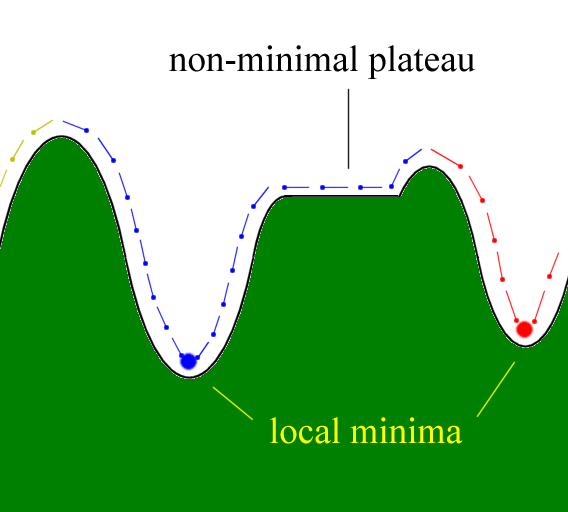
\includegraphics[height=5cm]{segmentation-watershed-rainfallingconcept-a.png}}%
	%
	\hspace{4mm}%
	%
	\subfigure[The division of the landscape into catchment basins]
	{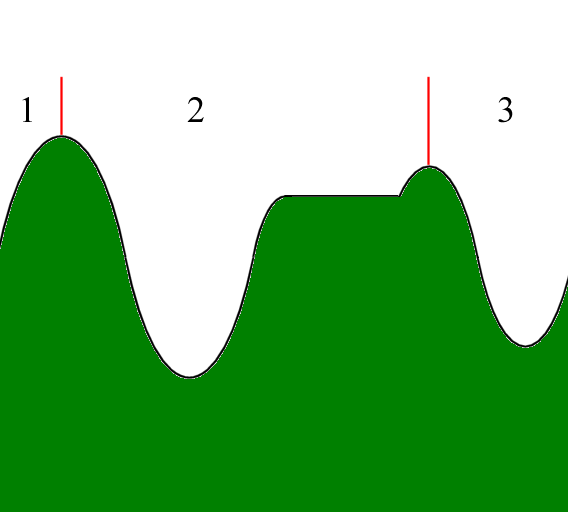
\includegraphics[height=5cm]{segmentation-watershed-rainfallingconcept-b.png}}%
\caption{The rainfalling concept of the watershed transform}
\label{fig:segmentation-watershed-rainfallingconcept}
\end{stusubfig}
%---

%---
\begin{stusubfig}{p}
	\subfigure[Beginning the flooding]
	{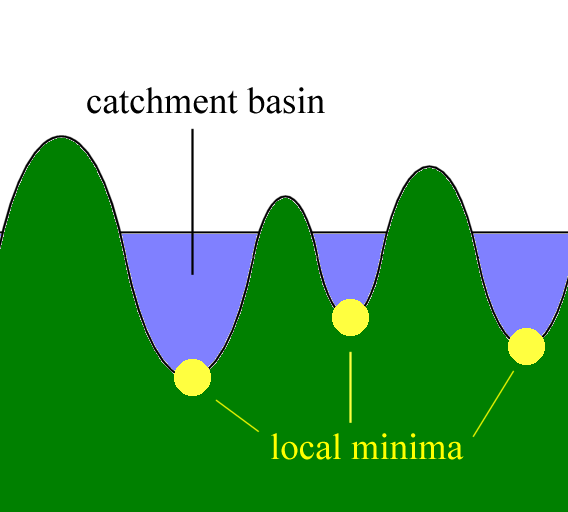
\includegraphics[height=5cm]{segmentation-watershed-floodingconcept-a.png}}%
	%
	\hspace{4mm}%
	%
	\subfigure[Two catchment basins meet]
	{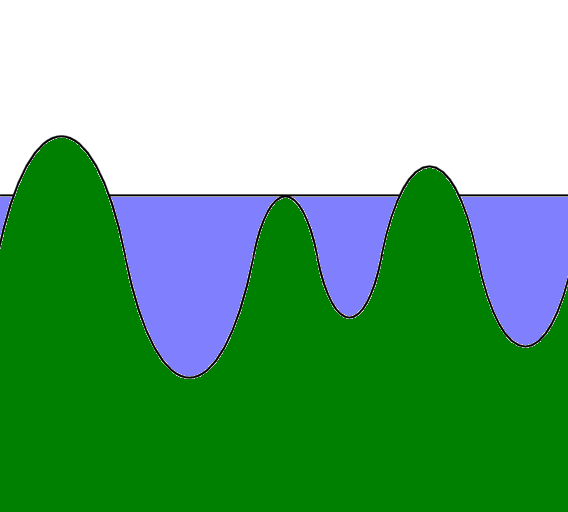
\includegraphics[height=5cm]{segmentation-watershed-floodingconcept-b.png}}%
	%
	\hspace{4mm}%
	%
	\subfigure[Building a watershed at the join point]
	{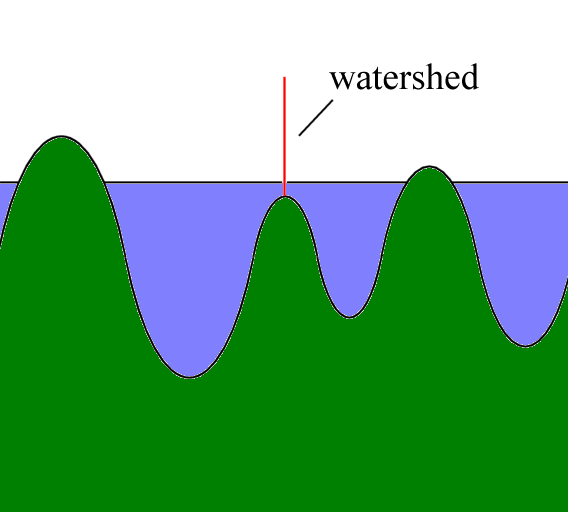
\includegraphics[height=5cm]{segmentation-watershed-floodingconcept-c.png}}%
	%
	\hspace{4mm}%
	%
	\subfigure[The division of the landscape into catchment basins]
	{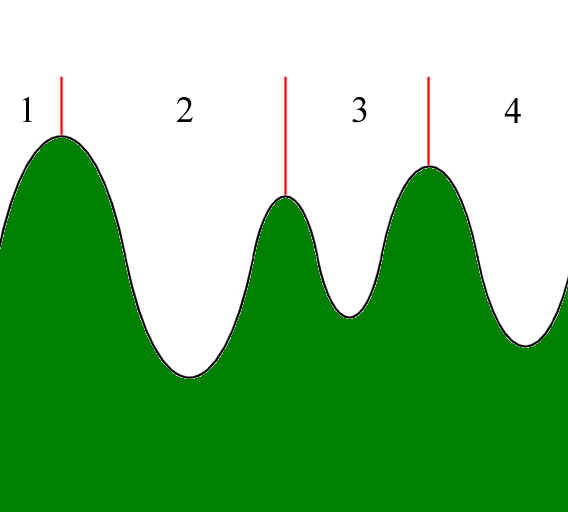
\includegraphics[height=5cm]{segmentation-watershed-floodingconcept-d.png}}%
\caption{The flooding concept of the watershed transform}
\label{fig:segmentation-watershed-floodingconcept}
\end{stusubfig}
%---

\noindent Image-based watershed methods produce a partition of their input into regions (see Figure~\ref{fig:segmentation-watershed-adfexample}). This can then be used for further processing.

%---
\begin{stusubfig}{t}
	\subfigure[The input image]
	{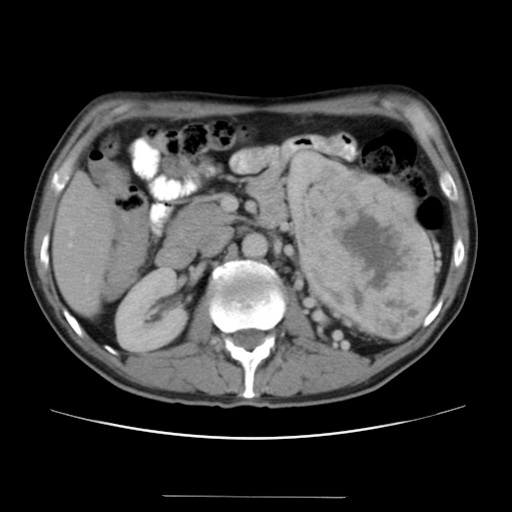
\includegraphics[height=5cm]{segmentation-watershed-adfexample-unsmoothed.png}}%
	%
	\hspace{4mm}%
	%
	\subfigure[The watershed of the image]
	{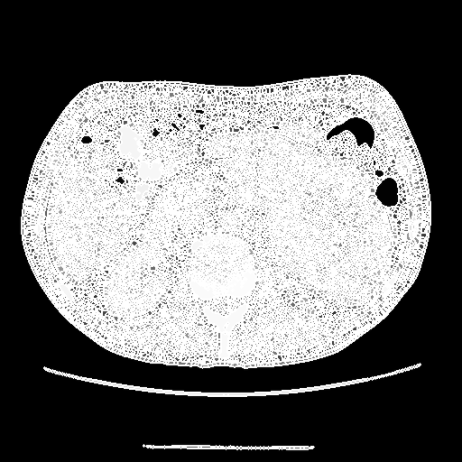
\includegraphics[height=5cm]{segmentation-watershed-adfexample-unsmoothedws.png}}%
\caption{The effects of the watershed transform. Note that the output is heavily over-segmented because the input is not smooth.}
\label{fig:segmentation-watershed-adfexample}
\end{stusubfig}
%---

\subsection{The Waterfall Transform}

In contexts where its input is not smooth (which amounts to the vast majority of real-world contexts), the watershed has an well-known and unfortunate tendency to produce an over-segmented output (again, see Figure~\ref{fig:segmentation-watershed-adfexample}). This is due to the presence of large numbers of spurious local minima in the input -- in conceptual terms, we are effectively segmenting a pock-marked landscape. The problem can be mitigated in various ways:
%
\begin{itemize}

\item The input can be smoothed (e.g.~using anisotropic diffusion filtering \cite{perona90}) before performing the watershed. This has the effect of removing some of the spurious local minima, but is usually not enough to actually solve the problem on its own. In practice, it often makes sense to smooth the image as a pre-processing step when applying hierarchical segmentation approaches -- note that this was done when producing Figure~\ref{fig:ipfs-ctconcept}, which is why the lowest partition of the image appears less over-segmented there than in Figure~\ref{fig:segmentation-watershed-adfexample}.

\item The watershed can be constrained using markers \cite{meyer90}. This directly tackles the problem by effectively specifying the desired number of output regions, but it imposes a significant manual input burden on the user.

\item The regions in the output can be iteratively merged together after finishing the watershed so as to construct a hierarchy of partitions of the input image. This does not reduce the over-segmentation of the lowest partition, but means instead that higher partitions may contain regions that are useful for later processing (e.g.~feature identification).

\end{itemize}
%
The waterfall transform is a multi-pass, hierarchical segmentation method that takes the third approach. As shown in Figure~\ref{fig:ipfs-ctconcept}, it generates a sequence of partitions of a landscape, each coarser (i.e.~containing fewer regions) than the one preceding it. Conceptually, each pass of the waterfall takes its input partition (Figure~\ref{fig:segmentation-waterfall-passconcept}(a)) and transforms it into a `stepped' landscape, where there is a step corresponding to each watershed boundary, with the height of the lowest pass point along that boundary (Figure~\ref{fig:segmentation-waterfall-passconcept}(b)). It then performs a watershed transform on this stepped landscape and outputs a coarser partition of the landscape as its result (Figure~\ref{fig:segmentation-waterfall-passconcept}(c)). This process can be repeated as long as the most recent partition has more than one catchment basin (Figures~\ref{fig:segmentation-waterfall-passconcept}(d) and (e)).

%---
\begin{stusubfig}{p}
	\subfigure[The initial partition output by the watershed]
	{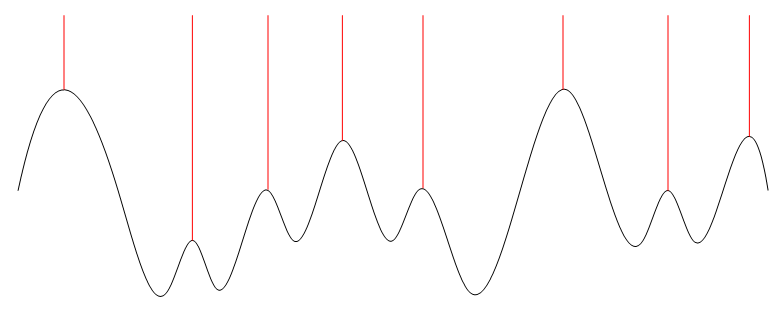
\includegraphics[height=3cm]{segmentation-waterfall-passconcept-a.png}}%
	%
	\hspace{4mm}%
	%
	\subfigure[After transforming it into a stepped landscape]
	{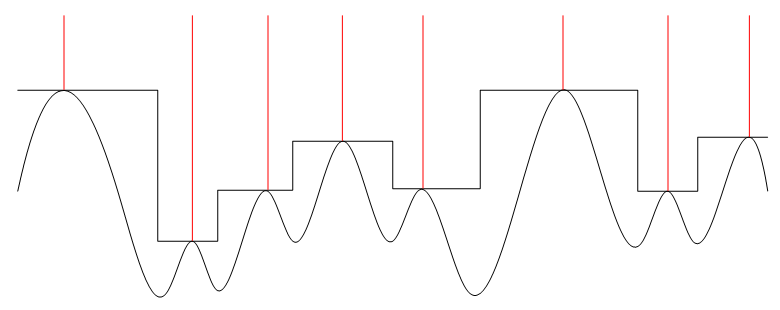
\includegraphics[height=3cm]{segmentation-waterfall-passconcept-b.png}}%
	%
	\hspace{4mm}%
	%
	\subfigure[After performing a watershed transform on the stepped landscape]
	{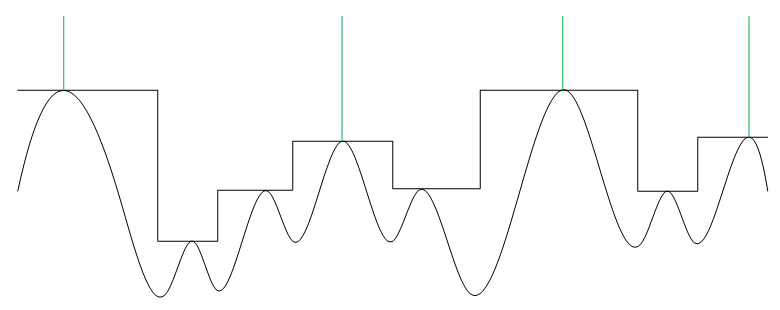
\includegraphics[height=3cm]{segmentation-waterfall-passconcept-c.png}}%
	%
	\hspace{4mm}%
	%
	\subfigure[After the second step transformation]
	{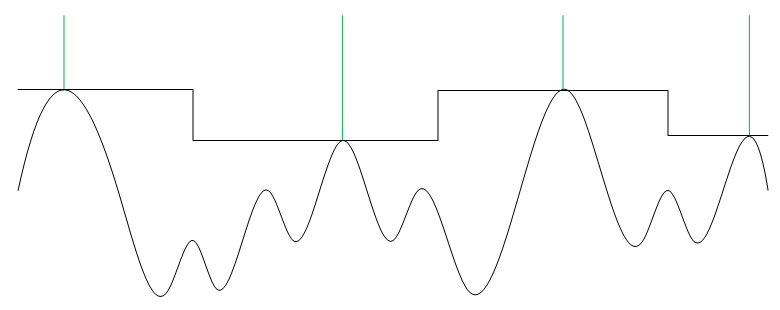
\includegraphics[height=3cm]{segmentation-waterfall-passconcept-d.png}}%
	%
	\hspace{4mm}%
	%
	\subfigure[After performing another watershed transform]
	{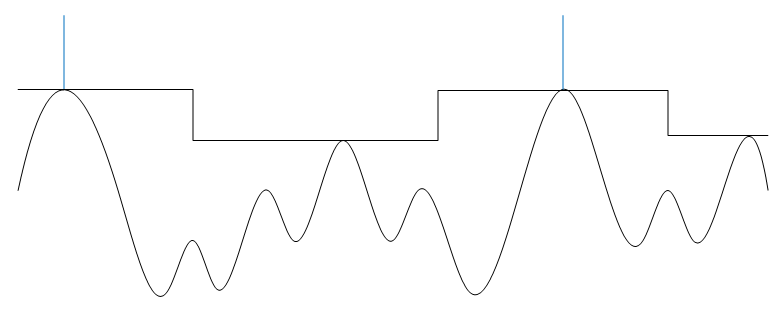
\includegraphics[height=3cm]{segmentation-waterfall-passconcept-e.png}}%
\caption{A conceptual view of the waterfall transform}
\label{fig:segmentation-waterfall-passconcept}
\end{stusubfig}
%---

\subsection{Marcotegui's Method}

Whilst it is possible to perform the waterfall using the conceptual approach just described, repeatedly transforming the landscape can potentially be costly -- e.g.~image-based methods for the waterfall have to process all of the pixels in each region rather than just processing the region itself. This militates for alternative approaches to the waterfall based on graphs -- these can be more efficient because an entire region can be represented by a single node.

Marcotegui's method \cite{marcotegui05} is a fast and effective example of such an approach. It works on a minimum spanning tree (MST) of the (weighted) region adjacency graph (RAG) of its input partition\footnotemark{}. The nodes of this graph correspond to regions in the input partition; its edges join adjacent nodes, and each edge is weighted with the height of the lowest pass point on the boundary between the nodes it joins.

\footnotetext{The justification for why an MST is sufficient can be found in \cite{marcotegui05}.}

At the start of Marcotegui's method, the first input partition (produced from the input using the watershed transform) is converted into its RAG representation in a straightforward manner and an MST is built from the RAG (see \S{}A.2 of \cite{golodetz11} for implementation details). This MST is then subjected to a sequence of waterfall passes. Each waterfall pass performs a flooding-based watershed on the MST to decide which regions should be merged and elides appropriate edges in the MST to effect this (eliding an an edge means combining the nodes at either end of the edge and removing the edge itself from the MST). In detail, this involves the following steps:
%
\begin{enumerate}

\item \emph{Determination of the local minima of the MST.} A local minimum of a weighted graph $G$ is a connected subgraph of $G$ whose edges have equal weight and whose adjacent edges in $G$ have strictly higher weights. Figure~\ref{fig:segmentation-waterfall-marcotegui-localminima}(a) shows an example graph and its local minima. Algorithmically, we iterate over the edges in the MST and flood out from each one to determine (a) whether it's part of a local minimum and (b) the extent of the minimum if so.

\item \emph{Elision of the local minima.} This is equivalent to merging minimal plateaux in a landscape into single points to which water runs down. See Figure~\ref{fig:segmentation-waterfall-marcotegui-localminima}(b). For clarity, we represent elision by assigning the nodes at the ends of an elided edge the same colour rather than removing the edge itself.

\item \emph{Propagation.} We flood out from the nodes that now represent the local minima (`marker nodes') along the edges, in non-decreasing order of edge weight, starting from the edges directly adjacent to the marker nodes. Each edge will either join a marker to a marker, in which case it should be ignored (since eliding it would merge two catchment basins), or it will join a marker to a non-marker, in which case it should be elided. See Figure~\ref{fig:segmentation-waterfall-marcotegui-propagation}.

\end{enumerate}

%---
\begin{stusubfig}{p}
  \subfigure[An example graph and its local minima (drawn in red)]
	{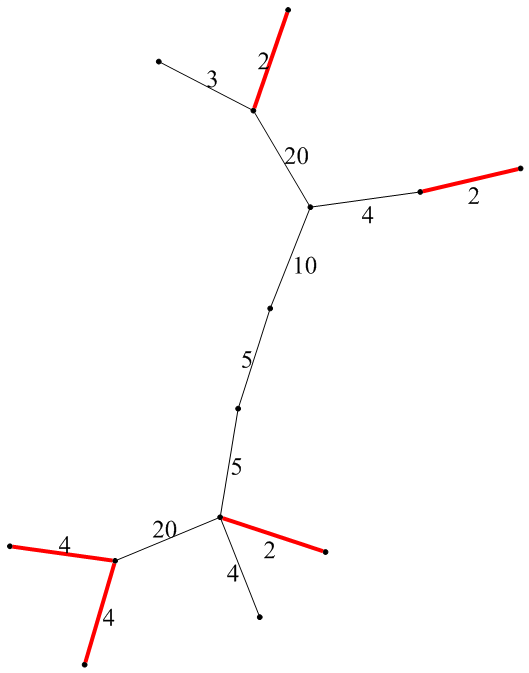
\includegraphics[width=.3\linewidth]{segmentation-waterfall-marcotegui-graphlocalminima.png}}%
	%
	\hspace{4mm}%
	%
	\subfigure[Eliding/colouring the local minima (the edges to be elided are drawn in blue)]
	{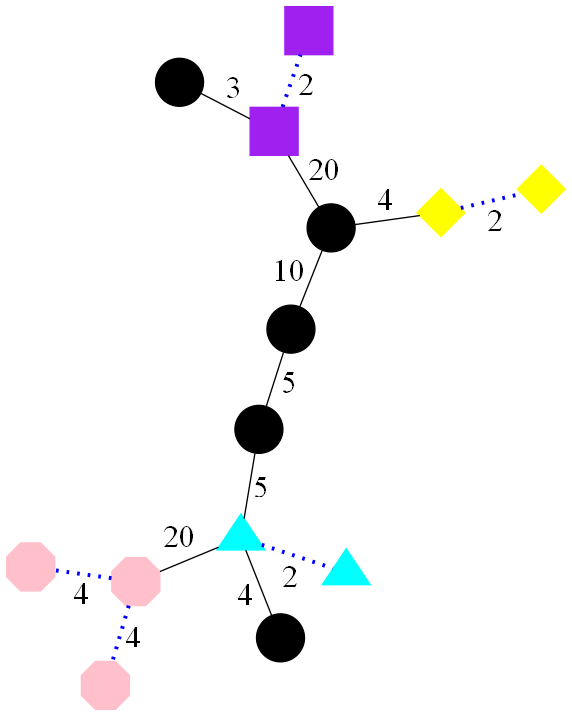
\includegraphics[width=.3\linewidth]{segmentation-waterfall-marcotegui-localminimaelision.png}}%	
\caption{Finding and eliding a graph's local minima for Marcotegui's method}
\label{fig:segmentation-waterfall-marcotegui-localminima}
\end{stusubfig}
%---

%---
\begin{stusubfig}{p}
	\subfigure[Initial state]
	{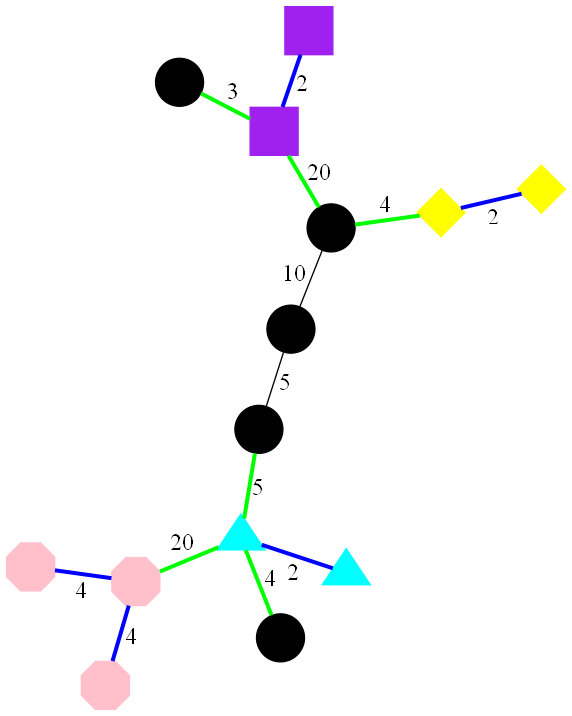
\includegraphics[width=.3\linewidth]{segmentation-waterfall-marcotegui-propagation-a.png}}%
	%
	\hspace{4mm}%
	%
	\subfigure[Elide the 3 edge]
	{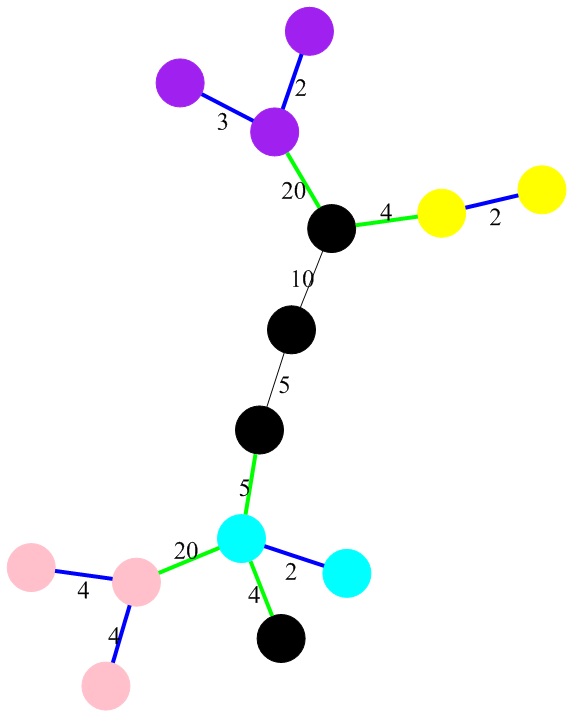
\includegraphics[width=.3\linewidth]{segmentation-waterfall-marcotegui-propagation-b.png}}%
	%
	\hspace{4mm}%
	%
	\subfigure[Elide a 4 edge]
	{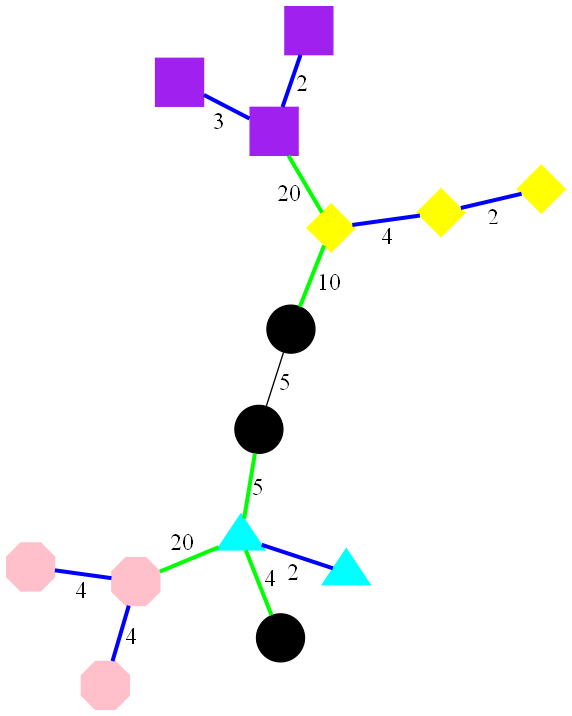
\includegraphics[width=.3\linewidth]{segmentation-waterfall-marcotegui-propagation-c.png}}%
	%
	\hspace{4mm}%
	%
	\subfigure[Elide another 4 edge]
	{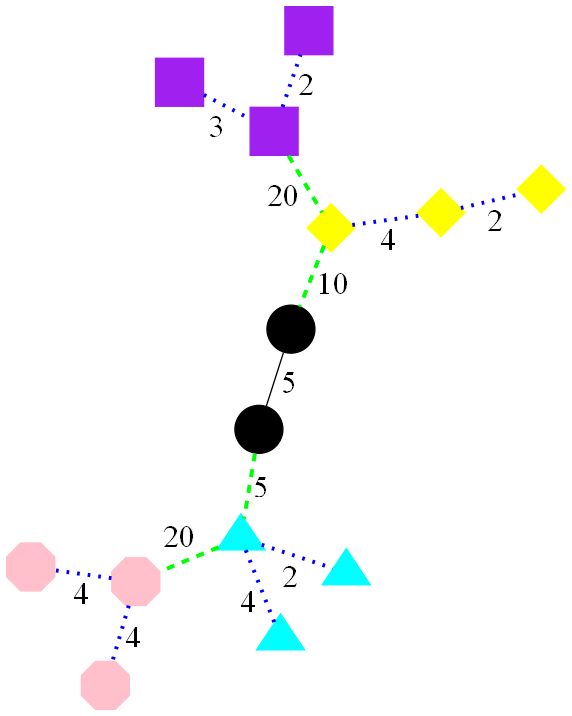
\includegraphics[width=.3\linewidth]{segmentation-waterfall-marcotegui-propagation-d.png}}%
	%
	\hspace{4mm}%
	%
	\subfigure[Elide the 5 edge]
	{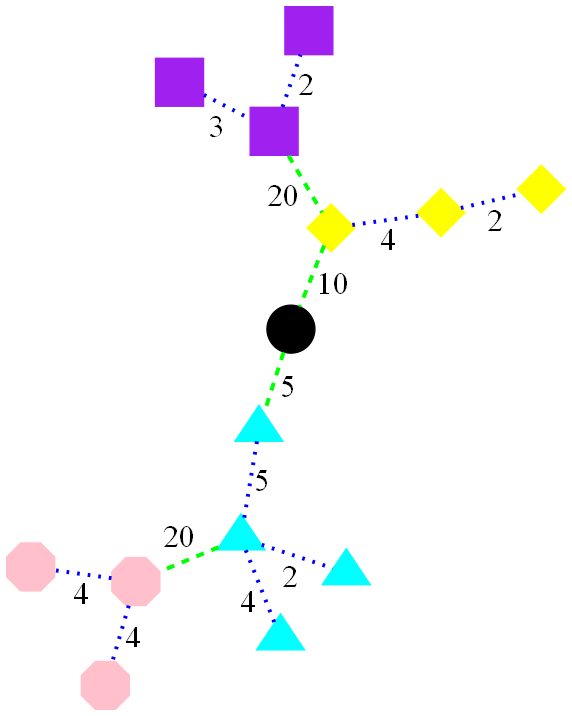
\includegraphics[width=.3\linewidth]{segmentation-waterfall-marcotegui-propagation-e.png}}%
	%
	\hspace{4mm}%
	%
	\subfigure[Elide the other 5 edge; all remaining edges will not be elided]
	{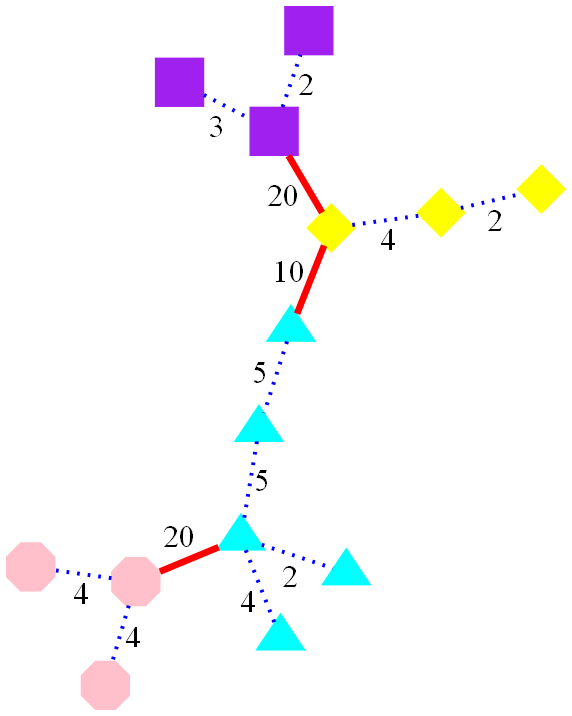
\includegraphics[width=.3\linewidth]{segmentation-waterfall-marcotegui-propagation-f.png}}%
\caption{The propagation step of Marcotegui's method, illustrated on the graph in \cite{marcotegui05}: blue edges have already been elided, green edges are under consideration, and red edges will not be elided.}
\label{fig:segmentation-waterfall-marcotegui-propagation}
\end{stusubfig}
%---

\noindent It is important to note that the order in which edges should be processed during the propagation step is not in general well-defined (note that multiple edges can have the same weight and thus be candidates for elision simultaneously). A straightforward implementation of the propagation step would use a priority queue and pop a lowest adjacent edge for consideration each time: thus the next edge to be considered ends up depending fundamentally on the way the priority queue is implemented. The consequence of this is that non-minimal plateaux in the MST are handled in a rather arbitrary way. This is not necessarily a problem in practice -- there tend to be only a small number of non-minimal plateaux in most MSTs, so it doesn't seriously affect the end result -- but it still seems undesirable to have the segmentation output depend so closely on the implementation of an internal data structure which may in principle be subject to change. This issue is dealt with robustly in \S\ref{sec:golodetz}.

%############################
\section{CN Method}
\label{sec:nicholls}
%############################

Despite the speed and effectiveness of Marcotegui's method, it can be somewhat intricate to implement \cite{golodetz08} because it is defined as a general graph method even though it operates on a tree. A simpler, tree-based method can be devised by observing that if an edge is not elided by a waterfall pass, it is because it is a highest edge separating two adjacent catchment basins (alternatively, it is a highest edge on the MST path between two adjacent local minima in the MST). Instead of explicitly finding the local minima in the graph and flooding out from them, it therefore suffices to root the MST somewhere and then work recursively up from the bottom of the tree, carefully maintaining a highest edge (`guard edge') guarding each local minimum encountered on the way.

%---
\begin{stusubfig}{p}
	\subfigure[Before rooting the MST]
	{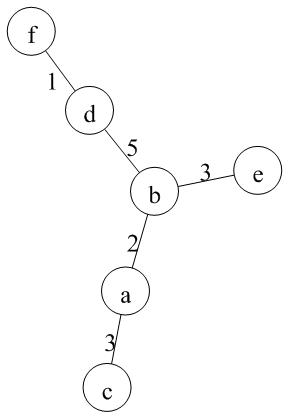
\includegraphics[height=5.5cm]{segmentation-waterfall-nicholls-root-before.png}}%
	%
	\hspace{4mm}%
	%
	\subfigure[After rooting it]
	{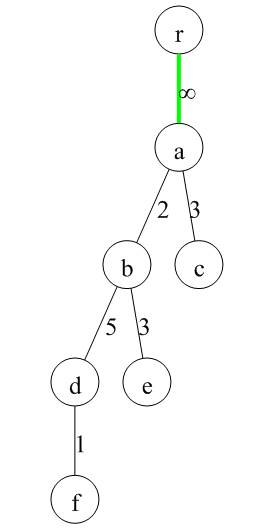
\includegraphics[height=5.5cm]{segmentation-waterfall-nicholls-root-after.png}}%
\caption{The CN method starts by picking a node at which to root the MST}% and adding a dummy root edge above the chosen root}
\label{fig:segmentation-waterfall-nicholls-root}
\end{stusubfig}
%---

The CN method initially roots the MST (see Figure~\ref{fig:segmentation-waterfall-nicholls-root}), adding a dummy `root edge' with a value strictly greater than the values of the edges descending from the root node (we will henceforth -- without ambiguity -- call edges descending from a node \emph{children} of the edge ascending from that node). The value chosen is unimportant, but $\infty$ or $1$ greater than the maximum value on a child edge are sensible choices. Each pass of the method is invoked on the root edge, and proceeds recursively as follows:
%
\begin{enumerate}

\item If the current edge is a leaf edge (i.e.~it has no child edges) then it is marked as a non-guard edge.

\item Otherwise:

\begin{enumerate}

\item We recurse on all the child edges.

\item A child edge with minimum value is chosen (if one or more of the children with minimum value is a guard edge, one of those is chosen in preference to a non-guard). This is then referred to as the `lowest child'. The value on the current edge is compared to the value on the lowest child. If its value is less than that of the lowest child, it is marked as a non-guard edge; otherwise it is marked as a guard and the lowest child is marked as a non-guard.

\item All non-guard children are then elided.

\end{enumerate}

\end{enumerate}

\noindent The workings of the method can be illuminated by a case analysis. There are two cases to consider: either the current edge (the parent edge) \emph{isn't} strictly the lowest leading out of a node, in which case at least part of the implied flow from the node is along the lowest child (see Figure~\ref{fig:segmentation-waterfall-nicholls-cases}(a)), or it is, in which case the implied flow from the node is entirely along the parent (see Figure~\ref{fig:segmentation-waterfall-nicholls-cases}(b)). In the first case, the method arbitrarily assumes that all the implied flow is along the lowest child. In both cases, the various child edges are then elided (or not) accordingly. Figure~\ref{fig:segmentation-waterfall-nicholls-example} illustrates how the method works on the same graph used to illustrate Marcotegui's method above.

%---
\begin{stusubfig}{p}
	\subfigure[The considered edge is not the unique lowest edge]
	{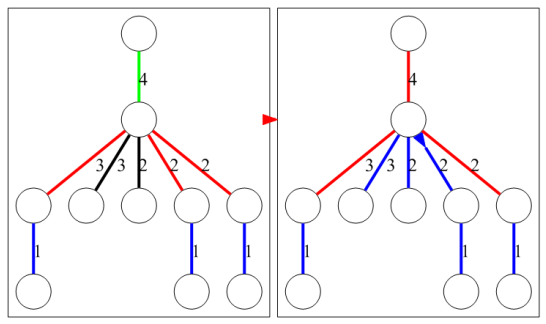
\includegraphics[height=4.5cm]{segmentation-waterfall-nicholls-cases-a.png}}%
	%
	\hspace{4mm}%
	%
	\subfigure[The considered edge is the unique lowest edge]
	{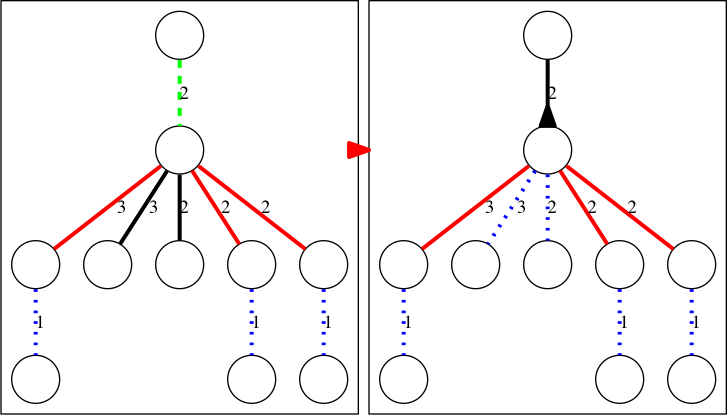
\includegraphics[height=4.5cm]{segmentation-waterfall-nicholls-cases-b.png}}%
\caption[Case analysis for the recursive step of the CN method]{Case analysis for the recursive step of the CN method: black edges are non-guards, red edges are guards, blue edges are those which have been elided and the green edge is the one under active consideration. The arrow (on the node) indicates the direction in which the method presumes water to flow.}
\label{fig:segmentation-waterfall-nicholls-cases}
\end{stusubfig}
%---

The assumption that all the implied flow is along the lowest child in the first case is this method's way of dealing with non-minimal plateaux in the MST. As with the Marcotegui method's dependence on the particular priority queue implementation used, this is a somewhat arbitrary way of handling non-minimal plateaux: in particular, the selected direction of implied flow from a particular node depends on both where the MST is rooted, and the specific method used to choose the lowest child. The method also ignores the possibility that part of the implied flow is along the parent. All of this affects which specific edges are elided. As with Marcotegui's method, this tends not to significantly degrade the end result, but it is still in principle desirable to devise a method that does not depend on such implementation details. In the following section, we therefore present an alternative tree-based method that handles non-minimal plateaux in the MST in a more robust manner.

%---
\begin{stusubfig}{p}
	\subfigure[Level 7]{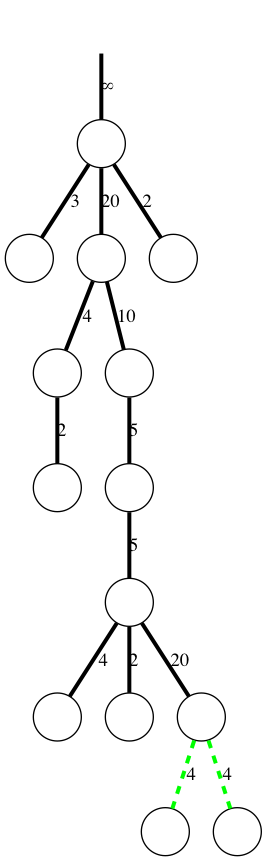
\includegraphics[width=.2\linewidth]{segmentation-waterfall-nicholls-example-a.png}}%
	\hspace{4mm}%
	\subfigure[Level 6]{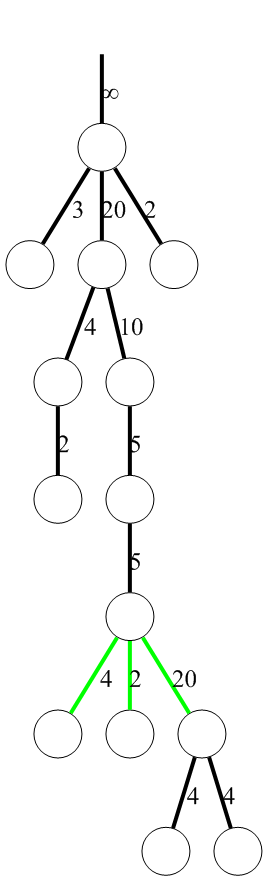
\includegraphics[width=.2\linewidth]{segmentation-waterfall-nicholls-example-b.png}}%
	\hspace{4mm}%
	\subfigure[Level 5]{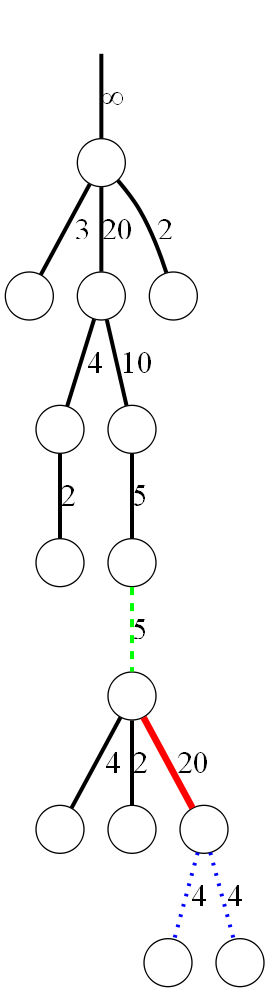
\includegraphics[width=.2\linewidth]{segmentation-waterfall-nicholls-example-c.png}}%
	\hspace{4mm}%
	\subfigure[Level 4]{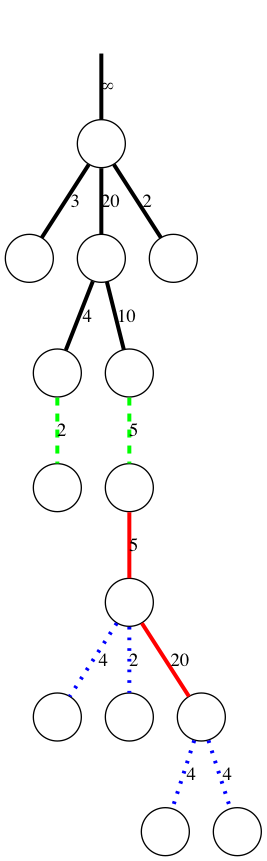
\includegraphics[width=.2\linewidth]{segmentation-waterfall-nicholls-example-d.png}}%
	\\
	\subfigure[Level 3]{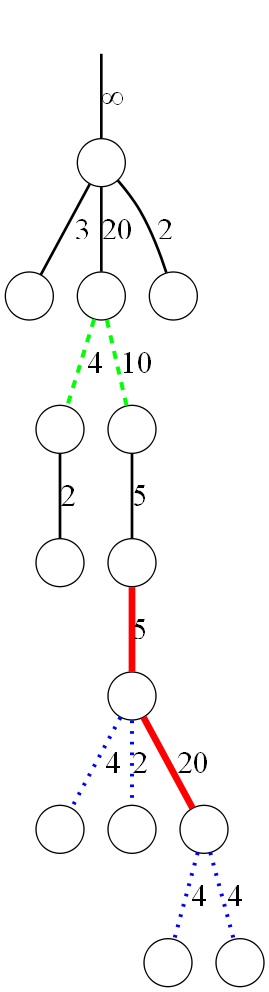
\includegraphics[width=.2\linewidth]{segmentation-waterfall-nicholls-example-e.png}}%
	\hspace{4mm}%
	\subfigure[Level 2]{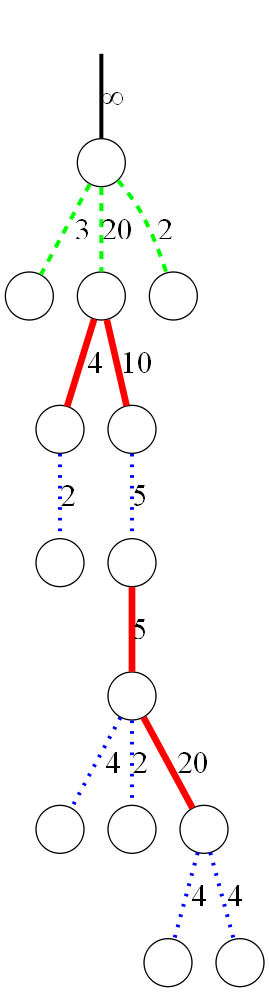
\includegraphics[width=.2\linewidth]{segmentation-waterfall-nicholls-example-f.png}}%
	\hspace{4mm}%
	\subfigure[Level 1]{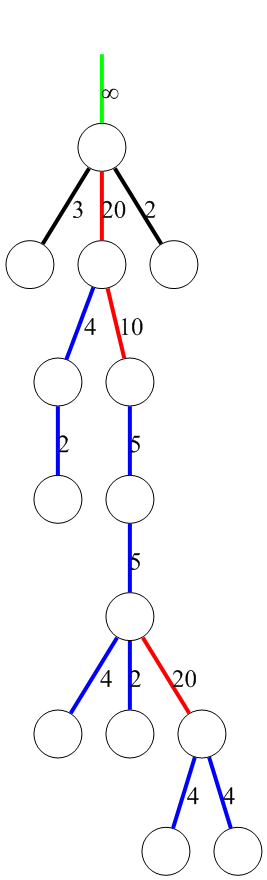
\includegraphics[width=.2\linewidth]{segmentation-waterfall-nicholls-example-g.png}}%
	\hspace{4mm}%
	\subfigure[Result]{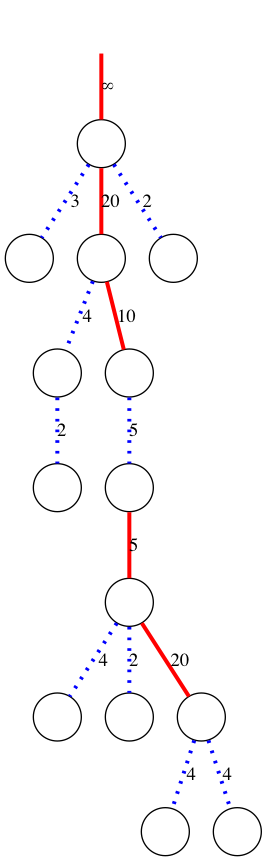
\includegraphics[width=.2\linewidth]{segmentation-waterfall-nicholls-example-h.png}}%
\caption[The CN method in action]{The CN method in action (considering all the edges in each level at a time for space reasons): black edges are non-guards, red edges are guards, blue edges are those which have been elided and green edges are ones under active consideration.}
\label{fig:segmentation-waterfall-nicholls-example}
\end{stusubfig}
%---

%#############################
\section{SG Method}
\label{sec:golodetz}
%#############################

In order to robustly account for non-minimal plateaux in the MST, we adopt an idea from Meijster and Roedink's image watershed algorithm \cite{meijster98}: if we transform the landscape to make it `lower-complete' (that is, we transform it into a landscape in which there is a unique path of steepest descent from each point), then the direction of flow is clear at every point and there is no ambiguity about how to assign non-minimal plateau points to catchment basins. The method for making the image lower-complete described in \cite{meijster98} has the effect of treating pixels that are further from the border of a plateau as being in some sense `higher' than those on the boundary. The same sort of idea can be applied in the context of a waterfall pass (although it is not necessary to actually transform the MST to make it lower-complete): where there are non-minimal plateaux in the MST, we can arrange to treat the nodes further from the border of the plateaux as being `higher` than their boundary counterparts. As we will see, this enables a robust decision to be made about which edges to elide.

The SG method is a tree-based, rainfalling approach and works in three recursive passes. The first pass works up the tree from the leaf nodes, marking initial path(s) of steepest from each node whilst allowing for the fact that they may need to be refined later. The second pass works down the tree from the root, updating the path(s) for each node to take account of routes via parent edges and marking edges for later elision as necessary. The final pass works up the tree again to actually elide the marked edges. (This cannot be done on a down pass for technical reasons.) The MST can be rooted anywhere in order to form the input tree -- the results are the same for any choice of root. In detail, the method works as follows:
%
\begin{enumerate}

\item \emph{Up Pass.} For each node, starting from the root:

\begin{enumerate}
\item Recursively process any children (the fact that the children are processed first is why this is called an `up' pass).
\item If this node has a unique edge of steepest descent (i.e.~a unique lowest-valued edge leading out of it, which can be the parent edge), add an arrow on the node pointing along the edge.
\item Otherwise, consider all the lowest-valued child edges (i.e.~ignore the parent for now, even if it is also a lowest-valued edge) that satisfy the condition that there is no arrow on the node at the other end of the edge pointing along the edge towards this node. If there are no such child edges, then this node is unescapable along a child edge and should be given a distance value of $\infty$. Otherwise, each of these child edges can be assigned a distance value equal to $1$ greater than the value on the node at the other end of the edge: this value on the node will be $0$ for nodes from which there is a unique path of steepest descent, and non-zero otherwise. Pick all the child edges whose distance value is minimal and add arrows from this node pointing along them (these indicate the initial paths of steepest descent from this node). Store the minimum distance value as this node's value.
\item Now consider the parent edge: if it was a lowest-valued edge, mark it as a potential path of steepest descent to avoid the need to check again in the second pass (in Figures~\ref{fig:segmentation-waterfall-smg-pass1cases}--\ref{fig:segmentation-waterfall-smg-example}, an open-headed arrow is used to mark a parent edge for later processing).
\end{enumerate}

\item \emph{Down Pass.} For each node, starting from the root:

\begin{enumerate}
\item \emph{Check upwards route.} If a node was marked as having a potential upwards path of steepest descent, first check to make sure that there is no arrow on the parent node pointing down the edge to this node. If not, there is a possible route upwards whose distance value is $1$ greater than the value on the parent node. This is compared to any existing routes downwards via child edges. If the upwards route is strictly better, the downwards arrows are removed, the upwards route is marked and the distance value on the node is updated to reflect the better route. If the upwards route is equally good, the parent edge is marked but no other changes are made. If the upwards route is worse, it is simply ignored.
\item \emph{Check whether the parent edge (if any) should be elided.} The decision on whether or not to elide an edge is based on a classification of its two end nodes with respect to the edge itself (this is why it can only be done at this point in the method). Nodes can be classified into one of five types with respect to the edge: unambiguous in (the flow from the node goes only along this edge), ambiguous in (part, but not all, of the flow from the node goes along this edge), unambiguous out (the flow from the node goes along precisely one of the other edges leading out of it), ambiguous out (the flow from the node goes along at least two of the other edges leading out of it) and no flow (there is no flow from the node at all). Based on these classifications, the parent edge is either marked for elision or not according to the case analysis shown in Figure~\ref{fig:segmentation-waterfall-smg-mergecases}. Note that there are only $13$ cases possible, rather than the expected $15$: \{ambiguous in, ambiguous in\} and \{ambiguous in, unambiguous in\} can never occur due to the way the method works.
\item \emph{Recurse on any children}.
\end{enumerate}

\item \emph{Up Pass.} Walk back up the tree to elide the marked edges.

\end{enumerate}

\noindent It is possible to perform a case analysis for the first pass and the route resolution step 2(a) as well (see Figures~\ref{fig:segmentation-waterfall-smg-pass1cases} and \ref{fig:segmentation-waterfall-smg-resolutioncases}), and this is helpful to clarify the workings of the method. Figure~\ref{fig:segmentation-waterfall-smg-example} illustrates how the method works on the now familiar graph used to demonstrate the workings of the previous two waterfall approaches.

%---
\begin{stusubfig}{p}
	\subfigure[UI/UI]{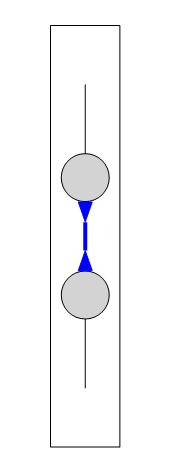
\includegraphics[height=5cm]{segmentation-waterfall-smg-mergecases-uiui.png}}%
	\hspace{4mm}
	\subfigure[UI/UO]{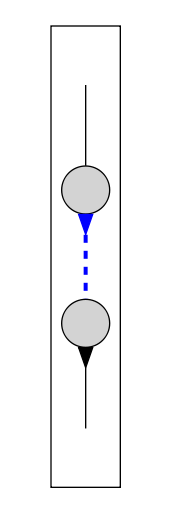
\includegraphics[height=5cm]{segmentation-waterfall-smg-mergecases-uiuo.png}}%
	\hspace{4mm}
	\subfigure[UO/AO]{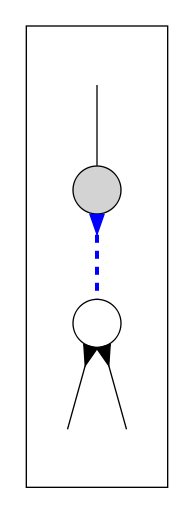
\includegraphics[height=5cm]{segmentation-waterfall-smg-mergecases-uiao.png}}%
	\hspace{4mm}
	\subfigure[UI/NF]{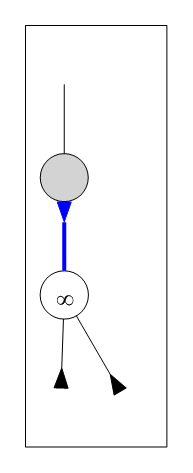
\includegraphics[height=5cm]{segmentation-waterfall-smg-mergecases-uinf.png}}%
	\hspace{4mm}
	\subfigure[NF/NF]{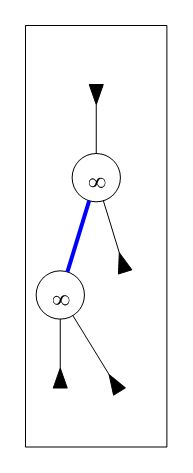
\includegraphics[height=5cm]{segmentation-waterfall-smg-mergecases-nfnf.png}}%
	\\
	\subfigure[UO/UO]{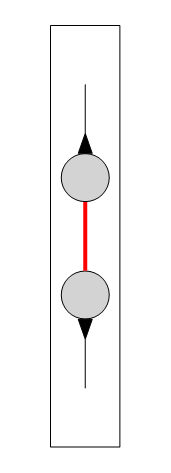
\includegraphics[height=5cm]{segmentation-waterfall-smg-mergecases-uouo.png}}%
	\hspace{4mm}
	\subfigure[UO/AI]{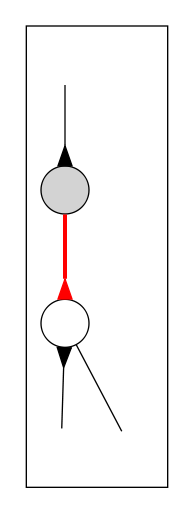
\includegraphics[height=5cm]{segmentation-waterfall-smg-mergecases-uoai.png}}%
	\hspace{4mm}
	\subfigure[UO/AO]{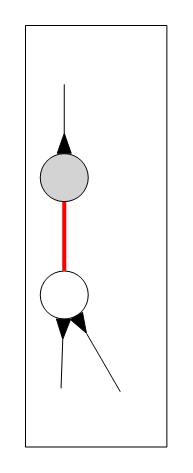
\includegraphics[height=5cm]{segmentation-waterfall-smg-mergecases-uoao.png}}%
	\hspace{4mm}
	\subfigure[UO/NF]{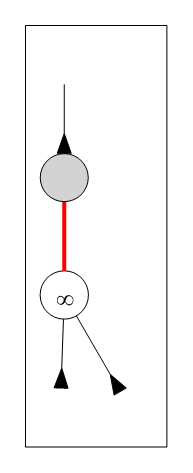
\includegraphics[height=5cm]{segmentation-waterfall-smg-mergecases-uonf.png}}%
	\\
	\subfigure[AO/AI]{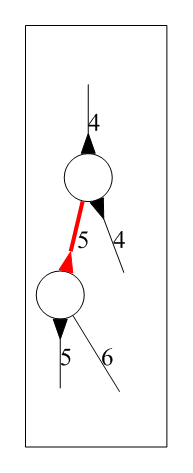
\includegraphics[height=5cm]{segmentation-waterfall-smg-mergecases-aoai.png}}%
	\hspace{4mm}
	\subfigure[AO/AO]{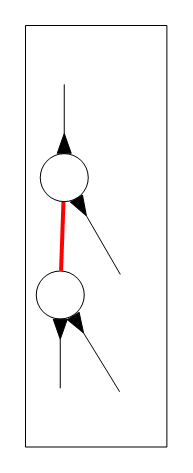
\includegraphics[height=5cm]{segmentation-waterfall-smg-mergecases-aoao.png}}%
	\hspace{4mm}
	\subfigure[NF/AI]{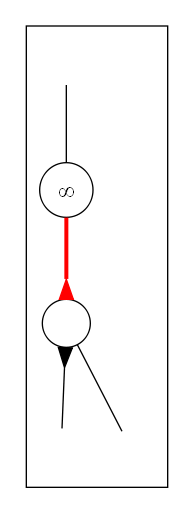
\includegraphics[height=5cm]{segmentation-waterfall-smg-mergecases-nfai.png}}%
	\hspace{4mm}
	\subfigure[NF/AO]{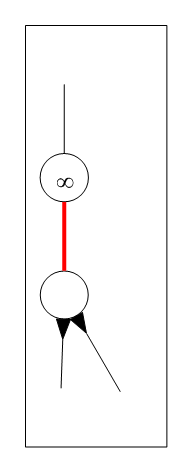
\includegraphics[height=5cm]{segmentation-waterfall-smg-mergecases-nfao.png}}%
\caption[Case analysis for the edge elision step of the SG method]{Case analysis for the edge elision step of the SG method (a blue edge indicates that the edge would be elided; a red edge indicates that it wouldn't). The labels are AI = ambiguous in, AO = ambiguous out, NF = no flow, UI = unambiguous in and UO = unambiguous out.}
\label{fig:segmentation-waterfall-smg-mergecases}
\end{stusubfig}
%---

%---
\begin{stusubfig}{p}
	\subfigure[The node has a unique path of steepest descent down a child edge]
	{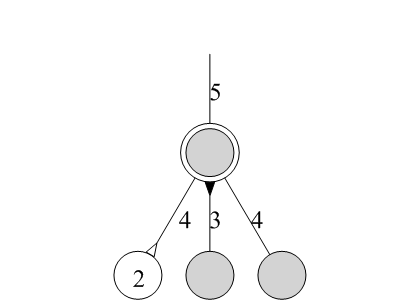
\includegraphics[width=.4\linewidth]{segmentation-waterfall-smg-pass1cases-a.png}}%
	%
	\hspace{4mm}%
	%
	\subfigure[The node has a unique path of steepest descent up the parent edge]
	{\includegraphics[width=.4\linewidth]{segmentation-waterfall-smg-pass1cases-b.png}}%
	%
	\hspace{4mm}%
	%
	\subfigure[The node has more than one path of steepest descent (and the parent edge is not a possible path of steepest descent)]
	{\hspace{8mm}\includegraphics[width=.4\linewidth]{segmentation-waterfall-smg-pass1cases-c.png}\hspace{8mm}}%
	%
	\hspace{4mm}%
	%
	\subfigure[The node has more than one \emph{downwards} path of steepest descent (but the parent edge still needs to be considered)]
	{\hspace{8mm}\includegraphics[width=.4\linewidth]{segmentation-waterfall-smg-pass1cases-d.png}\hspace{8mm}}%
	%
	\hspace{4mm}%
	%
	\subfigure[There is no flow out of the node]
	{\includegraphics[width=.4\linewidth]{segmentation-waterfall-smg-pass1cases-e.png}}%
	%
	\hspace{4mm}%
	%
	\subfigure[There is no downwards flow out of the node (but the parent edge still needs to be considered)]
	{\hspace{8mm}\includegraphics[width=.4\linewidth]{segmentation-waterfall-smg-pass1cases-f.png}\hspace{8mm}}%
\caption{Case analysis for the first pass of the SG method}
\label{fig:segmentation-waterfall-smg-pass1cases}
\end{stusubfig}
%---

%---
\begin{stusubfig}{p}
	\subfigure[The arrow from the parent node points towards us]
	{\includegraphics[height=5.5cm]{segmentation-waterfall-smg-resolutioncases-a.png}}%
	%
	\hspace{4mm}%
	%
	\subfigure[There is no flow from the parent node]
	{\includegraphics[height=5.5cm]{segmentation-waterfall-smg-resolutioncases-b.png}}%
	%
	\hspace{4mm}%
	%
	\subfigure[There is an equally good route via the parent node]
	{\includegraphics[height=5.5cm]{segmentation-waterfall-smg-resolutioncases-c.png}}%
	%
	\hspace{4mm}%
	%
	\subfigure[There is a better route via the parent node]
	{\includegraphics[height=5.5cm]{segmentation-waterfall-smg-resolutioncases-d.png}}%
\caption[Case analysis for the resolution step of the SG method]{Case analysis for the resolution step of the SG method (the circled node is the one currently under consideration in each case)}
\label{fig:segmentation-waterfall-smg-resolutioncases}
\end{stusubfig}
%---

%---
\begin{stusubfig}{p}
	\subfigure[The initial tree]{\includegraphics[width=.3\linewidth]{segmentation-waterfall-smg-example-initial.png}}%
	\hspace{4mm}%
	\subfigure[After the first pass]{\includegraphics[width=.3\linewidth]{segmentation-waterfall-smg-example-pass1.png}}%
	\hspace{4mm}%
	\subfigure[After the second pass]{\includegraphics[width=.3\linewidth]{segmentation-waterfall-smg-example-pass2.png}}%
\caption[The SG method running on a real example]{The SG method running on a real example: the arrows on the nodes indicate the flow direction, blue edges are those that will be elided and red edges are those that won't be.}
\label{fig:segmentation-waterfall-smg-example}
\end{stusubfig}
%---

%######################
\section{Experiments}
\label{sec:experiments}
%######################

We implemented all three methods (Marcotegui, CN and SG) in \emph{millipede} \cite{millipede}, our software for 3D abdominal CT image segmentation, feature identification and visualisation. The way in which we implemented Marcotegui's method in \emph{millipede} was a refinement of our initial approach that we described in \cite{golodetz08} -- in particular, the new implementation of the step that finds the local minima in the MST uses the first two passes of the SG method as an edge classifier (the local minima are those edges classified as either \{unambiguous in, unambiguous in\}, \{unambiguous in, no flow\} or \{no flow, no flow\}). This is a more efficient way of finding the local minima than the flooding approach described in \cite{golodetz08}.

\subsection{Output}

In order to compare the outputs of the methods, we ran each of them on three well-known test images from the computer vision field (see Figure~\ref{fig:testimages}). In each case, the input image was initially smoothed using anisotropic diffusion filtering \cite{perona90}. The first output partition in each case was produced using our implementation of Meijster and Roerdink's watershed algorithm \cite{meijster98}. The output partitions were compared by producing difference images using ImageMagick \cite{imagemagick}. The results are shown in Figures~\ref{fig:results-lena}--\ref{fig:results-peppers}.

The outputs of the methods are similar, as we would expect, but there are differences due to the ways in which the different methods handle non-minimal plateaux. We observe in particular that the outputs of the Marcotegui and SG methods are closer than those of the CN method and either of the other two methods. However, for the purpose of feature identification, all three methods produce results that are effectively equivalent.

%---
\begin{stusubfig}{p}
	\subfigure[Lena]{\includegraphics[width=.3\linewidth]{lena.png}}%
	\hspace{4mm}%
	\subfigure[Baboon]{\includegraphics[width=.3\linewidth]{baboon.png}}%
	\hspace{4mm}%
	\subfigure[Peppers]{\includegraphics[width=.3\linewidth]{pepper.png}}%
\caption{The three test images used to compare the methods}
\label{fig:testimages}
\end{stusubfig}
%---

%---
\begin{stusubfig}{p}
	\subfigure[Marcotegui]{\includegraphics[width=.3\linewidth]{lena-partition-3-M.png}}%
	\hspace{4mm}%
	\subfigure[CN Method]{\includegraphics[width=.3\linewidth]{lena-partition-3-NC.png}}%
	\hspace{4mm}%
	\subfigure[SG Method]{\includegraphics[width=.3\linewidth]{lena-partition-3-G.png}}%
	\\
	\subfigure[CN vs. SG]{\includegraphics[width=.3\linewidth]{lena-diff-3-GNC.png}}%
	\hspace{4mm}%
	\subfigure[Marcotegui vs. CN]{\includegraphics[width=.3\linewidth]{lena-diff-3-MNC.png}}%
	\hspace{4mm}%
	\subfigure[Marcotegui vs. SG]{\includegraphics[width=.3\linewidth]{lena-diff-3-GM.png}}%
\caption[]{Comparing the third partition produced by each of the methods for Lena. The top row shows the results produced by each method. The bottom row highlights the differences between the results.}
\label{fig:results-lena}
\end{stusubfig}
%---

%---
\begin{stusubfig}{p}
	\subfigure[Marcotegui]{\includegraphics[width=.3\linewidth]{baboon-partition-3-M.png}}%
	\hspace{4mm}%
	\subfigure[CN Method]{\includegraphics[width=.3\linewidth]{baboon-partition-3-NC.png}}%
	\hspace{4mm}%
	\subfigure[SG Method]{\includegraphics[width=.3\linewidth]{baboon-partition-3-G.png}}%
	\\
	\subfigure[CN vs. SG]{\includegraphics[width=.3\linewidth]{baboon-diff-3-GNC.png}}%
	\hspace{4mm}%
	\subfigure[Marcotegui vs. CN]{\includegraphics[width=.3\linewidth]{baboon-diff-3-MNC.png}}%
	\hspace{4mm}%
	\subfigure[Marcotegui vs. SG]{\includegraphics[width=.3\linewidth]{baboon-diff-3-GM.png}}%
\caption[]{Comparing the third partition produced by each of the methods for Baboon.}
\label{fig:results-baboon}
\end{stusubfig}
%---

%---
\begin{stusubfig}{p}
	\subfigure[Marcotegui]{\includegraphics[width=.3\linewidth]{pepper-partition-3-M.png}}%
	\hspace{4mm}%
	\subfigure[CN Method]{\includegraphics[width=.3\linewidth]{pepper-partition-3-NC.png}}%
	\hspace{4mm}%
	\subfigure[SG Method]{\includegraphics[width=.3\linewidth]{pepper-partition-3-G.png}}%
	\\
	\subfigure[CN vs. SG]{\includegraphics[width=.3\linewidth]{pepper-diff-3-GNC.png}}%
	\hspace{4mm}%
	\subfigure[Marcotegui vs. CN]{\includegraphics[width=.3\linewidth]{pepper-diff-3-MNC.png}}%
	\hspace{4mm}%
	\subfigure[Marcotegui vs. SG]{\includegraphics[width=.3\linewidth]{pepper-diff-3-GM.png}}%
\caption[]{Comparing the third partition produced by each of the methods for Peppers.}
\label{fig:results-peppers}
\end{stusubfig}
%---

\subsection{Timings}

In order to evaluate how well the methods scale with increasing input size, we timed each of them when used to segment increasingly large sub-images from a 3D abdominal CT scan\footnotemark{}. The overall scan was of size $512 \times 512 \times 132$, and we tested the methods on sub-images of size $512 \times 512 \times n$, for various different values of $n$. There was an upper bound of $n \le 40$ due to memory constraints. The experiment was run on a single 2.4GHz Pentium 4 CPU. Unlike in the previous experiment, in this experiment the input image was not smoothed (since smoothing is time-consuming and affects each method equally). The first output partition was again produced using the Meijster/Roerdink watershed. The results are shown in Figure~\ref{fig:timings}.

TODO

%---
\stufigex{width=.95\linewidth}{timings.png}{Timing results for the three methods on sub-images of an abdominal CT scan. The experiment was run on a single 2.4GHz Pentium 4 CPU. The overall scan was of size $512 \times 512 \times 132$, and each point on the graph represents how long (in seconds) a specific method took to run on a sub-image of size $512 \times 512 \times n$.}{fig:timings}{!t}
%---

\iffalse
%---
\begin{table}
\begin{center}
\begin{tabular}[p]{c||c|c|c}
& \multicolumn{3}{c}{\textbf{Time} (s)} \\
\textbf{Slices} ($n$) & \textbf{Marcotegui} & \textbf{CN} & \textbf{SG} \\
\hline
 5 & ? & ? & ? \\
10 & ? & ? & ? \\
20 & ? & ? & ? \\
40 & ? & ? & ?
\end{tabular}
\end{center}
\caption{Timing results for the three methods on sub-images of an abdominal CT scan. The experiment was run on a single 2.4GHz Pentium 4 CPU. The overall scan was of size $512 \times 512 \times 132$, and each line in the table represents how long (in seconds) each of the methods took to run on a sub-image of size $512 \times 512 \times n$.}
\label{tbl:results-time}
\end{table}
%---
\fi

\footnotetext{Specifically, this was the `BT' scan we obtained from the Churchill Hospital, Oxford.}

%#####################
\section{Discussion}
\label{sec:discussion}
%#####################

TODO

%######################
\section{Conclusions}
\label{sec:conclusions}
%######################

In this paper, we have introduced two new, tree-based methods for the classical waterfall transform from mathematical morphology and compared them with both the existing state-of-the-art and each other. The CN method is single-pass and is significantly easier to implement than the existing state-of-the art: indeed, it can be implemented using a single, short, recursive function. The SG method is slightly harder to implement (although still easier than previous methods), but deals consistently with the problem of non-minimal plateaux in the MST, something neither of the two other methods attempts. TODO

\clearpage

\bibliographystyle{alpha}
\bibliography{existingwork,mypapers}

\end{document}
